% В этом шаблоне используется класс spbau-diploma. Его можно найти и, если требуется, 
% поправить в файле spbau-diploma.cls
\documentclass{spbau-diploma}
\begin{document}
\filltitle{ru}{
    chair              = {Кафедра математических и информационных технологий},
    title              = {Анализ смесей близкородственных
бактериальных штаммов в метагеномных~сериях},
    type               = {master},
    position           = {студента},
    group              = 605,
    author             = {Аксешина Маргарита Дмитриевна},
    supervisorPosition = {},
    supervisor         = {Нурк С.\,Ю.},
    reviewerPosition   = {к.\,т.\,н},
    reviewer           = {Казаков С.\,В.},
    chairHeadPosition  = {д.\,ф.-м.\,н., профессор},
    chairHead          = {Омельченко А.\,В.},
}
\filltitle{en}{
    chair              = {Department of Mathematics and Information Technology},
    title              = {Analyzing mixtures of closely related strains in metagenomic series data},
    author             = {Margarita Akseshina},
    supervisorPosition = {},
    supervisor         = {Sergey Nurk},
    reviewerPosition   = {Ph.\,D.},
    reviewer           = {Sergey Kazakov},
    chairHeadPosition  = {professor},
    chairHead          = {Alexander Omelchenko},
}


\maketitle


\tableofcontents


% ВВЕДЕНИЕ
\section*{Введение}

\subsection{Введение в область} 
Метагеномика  изучает микробные сообщества, посредством секвенирования ДНК, полученной непосредственно из образцов среды, минуя этапы выделения и культивирования микроорганизмов. Метагеномика позволяет исследовать, как видовое, так и функциональное разнообразие микробных сообществ. Например, средствами метагеномики можно отслеживать, как меняется и от чего зависит такая важная часть здоровья человека, как его микробиом \cite{HMP1, HMP2}. Кроме того метагеномика предоставляет доступ к геномам микроорганизмов, которые на данный момент не поддаются культивации.

Активному развитию метагеномики в последнее десятилетие в значительной степени способствовало появление методов секвенирования нового поколения. Их результатом является набор коротких (обычно 100-250 нуклеотидов) геномных фрагментов -- \textit{ридов}. 
Отметим, что многие современные исследования включают анализ множества образцов, формирующих \textit{метагеномные серии} (пробы одного и того же сообщества, полученные в разные момент времени \cite{time_series} или в близких локациях ~\cite{spacial_series_1, spacial_series_2}.

Важные функциональные элементы генома (гены, регуляторные участки, повторы и т.д.) обычно не умещаются в один рид. 
С целью проведения дальнейшего анализа многие современные исследования предварительно объединяют риды в более длинные последовательности исходных геномов -- \textit{контиги}. Для этого используются специализированные программные инструменты -- метагеномные сборщики (\cite{IDBA-UD, MEGAHIT, MetaVelvet, RayMeta, MetaSpades}). При этом риды метагеномных серий можно объединять и собирать вместе, чтобы повысить покрытие малопредставленных организмов. 

За этапом сборки обычно следует этап \textit{биннинга}, -- то есть разделение полученных контигов на группы, в идеале соответствующие отдельным микроорганизмам. Инструменты для биннинга \cite{CONCOCT, GroopM, MyCC, MetaBAT} основываются на анализе состава нуклеотидных последовательностей (например, тетрануклеотидном <<спектре>>), а также глубины их покрытия в образце (или каждом из образцов серии, при наличии таковых). 


\subsection{Штаммы близкородственных видов}


Заметим, что можно изучать микроорганизмы не на уровне видов, а ниже --- на уровне штаммов. Важным преимуществом данного подхода над методами метагеномного анализа видового состава образцов является возможность функциональной аннотации генома конкретной популяции того или иного вида, присутствующего в данном образце. Различные штаммы одного вида микроорганизма могут сильно отличаться по своим функциональным свойствам (включая патогенность, вирулентность и резистентность к антибиотикам).

К сожалению, ситуация значительно усложняется  в случае, если в одном образце присутствует несколько штаммов одного вида \cite{StrainEst, metasub, infant_gut}.
В этом случае, за счет чередования в их геномах консервативных и вариабельных участков, итоговый набор контигов оказывается сильно фрагментированным. При этом, существующие процедуры биннинга оказываются неспособны как декомпозировать этот набор на (пересекающиеся (???)) кластера, соответствующие индивидуальным штаммам, так и корректно выделить набор контигов, соответствующих их объединению (все контиги для данного вида микроорганизма).

Важное понимать, что в метагеномной серии процентное соотношение близкородственных штаммов определенной микробной популяции (вида) может существенно изменяться от образца к образцу. Помимо того, что подобные изменения представляют значительный биологический интерес, они также дают дополнительную информацию для более глубокого анализа композиции и свойств индивидуальных штаммов.

Наиболее передовым методом подобного анализа смесей близкородственных штаммов является DESMAN \cite{DESMAN}.
Подобно более ранним работам (ConStrains \cite{Constrains}, Lineage \cite{Lineage}), в его основе лежит анализ частот однонуклеотидных замен (Single Nucleotide Variant frequency), относительно выравнивания на некоторую референсную последовательность (или набор последовательностей, в первую очередь генов) для интересующего вида. 
В данном случае под частотой мутации понимается доля ридов, поддерживающих данную мутацию. 
Если мутация относительно определенной позиции референса присутствует только в одном из штаммов, её профиль частот в образцах будет соответствовать частоте этого штамма (Рис. \ref{snv_profile}, первая SNV). 
Однако если мутация присутствует в нескольких штаммах, все они будут вносить вклад в её профиль частот (Рис. \ref{snv_profile}, вторая SNV). 
Заметим, что подобные рассуждения могут применяться, только к регионам, присутствующим во всех штаммах и не являющихся геномными повторами (Рис. \ref{snv_profile}, третья SNV). 
% * <novmargo@gmail.com> 11:34:25 09 Jun 2018 UTC+0300:
% (ПОЯСНИТЬ ЧТО ТАКОЕ ПРОФИЛЬ)


\begin{figure}[t]
\centering
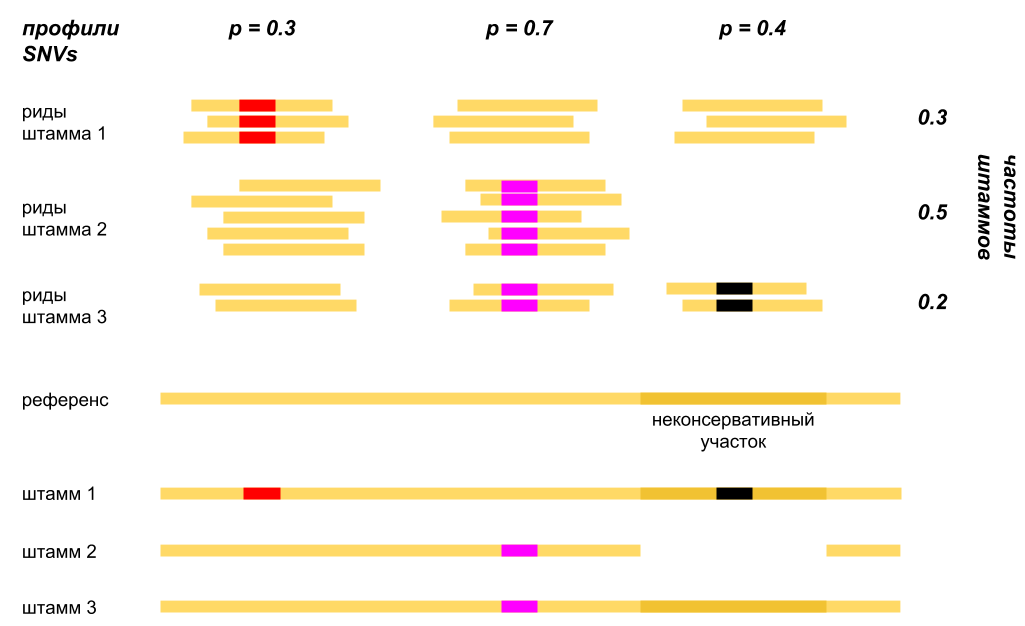
\includegraphics[width=0.9\textwidth]{pics/snv_profiles.png}
\caption{Подсчёт частот однонуклеотидныx мутаций (SNVs) для одного образца}
\label{snv_profile}
\end{figure}

 
Перед тем, как использовать DESMAN для анализа штаммов определенного микроорганизма, пользователь должен тем или иным способом выявить набор последовательностей (контигов или генов), соответствующих ему.
DESMAN детектирует SNV относительно однокопийных консервативных генов (которые скорее всего присутствуют в каждом из штаммов в единственном экземпляре). 
Затем на основании частот SNV с привлечением Байесовской модели выводится предполагаемое количество штаммов и профили глубины их покрытия. 
На следующем этапе для каждого из неконсервативных генов (тех, которые могут отсутствовать в одном или нескольких штаммах) DESMAN предсказывает подмножество включающих его штаммов.
%Отметим, что возможность определения генетического состава индивидуальных штаммов выделяет DESMAN...TODO if needed :). 

\subsection{Цель работы}
Целью данной работы является разработка пайплайна, который будет выявлять количество близкородственных штаммов в метагеномной серии, их процентное соотношение, а также для вершин графа сборки этих штаммов будет определять, какому подмножеству штаммов они принадлежат. 
Для решения последней задачи кроме информации о покрытии мы будем использовать ещё и информацию о структуре графа метагеномной сборки. 

%\subsection{Методы}
\subsection{Графы сборки}

\textit{Графом де Брюина}, построенном по множеству строк S, называется граф, вершины которого соответствуют всем возможным (k+1)-мерам (последовательность из k+1 символов), присутствующим в S, а направленное ребро соединяет вершину $A$ с вершиной $B$ в том и только том случае, если последние $k$ символов вершины $A$ равны первым $k$ символам вершины $B$.

\textit{Сжатым графом де Брюина} будем называть граф, получаемый из графа де Брюина путём итеративного объединения всех таких пар вершин (u, v) таких что из u выходит единственное ребро, идущее в v, которое также является единственным входящим ребром для v. Вершины u и v удаляются из графа, и добавляется новая вершина w, входящие рёбра которой равны входящим рёбрам u, исходящие -- исходящим рёбрам v. Последовательность символов, соответствующая w, получается путём присоединения к последовательности u всех символов v, кроме первых k.

Значительно упрощая, можно считать, что граф, с которым в дальнейшем предстоит работать (граф сборки) строится 
следующим образом:
\begin{enumerate}
    \item по множеству ридов строится граф де Брюина;
    \item по графу де Брюина строится сжатый граф де Брюина;
    \item так как в ридах содержатся ошибки секвенирования, далее сжатый граф де Брюина упрощается, чтобы по возможности удалить из графа структуры, порождаемые этими ошибками.
\end{enumerate}
Последовательности, соответсвующие вершинам в графе сборки, называются \textit{юнитигами}.

Если все участки генома были покрыты ридами, а в процессе упрощения графа были выкинуты только ошибочные вершины, то в графе существует путь, последовательность юнитигов которого соответствует геному. После построения графа сборки сборщики ищут такие пути или хотя бы их фрагменты, чтобы объединить юнитиги в более длинные последовательности --- \textit{контиги}.

%На сегодняшний момент нам известен только один инструмент, использующий структуру графа сборки для анализа смесей близкородственных штаммов, --- это MaryGold \cite{MaryGold}, но он только ищет набор мест в графе, соответствующих вариациям между штаммами. 



\section{Краткое описание подхода}

В данной работе мы будем анализировать графы сборки, полученные с помощью программы metaSPAdes \cite{MetaSpades}. Настройки этапа <<упрощения>> графа были модифицированы с целью сохранения связей между элементами, соответствующими различным штаммам (по-умолчанию metaSPAdes стремится в первую очередь обеспечить реконструкцию наиболее высоко-представленного штамма). 

В начале мы используем DESMAN для того, чтобы найти количество штаммов и их процентное соотношение. 

Далее мы используем модуль gene-assign программы DESMAN, чтобы определить, каким штаммам принадлежат вершины графа сборки, соответствующие длинным юнитигам геномов. Введение порогового значения на минимальную длину (в текущих экспериментах 1кб) позволяет: 
\begin{enumerate}
    \item исключить из рассмотрения большинство геномных повторов (CСЫЛКА);
    \item обеспечить более точное соответствие средней глубины покрытия рассматриваемых вершин среднему значению по геному.
\end{enumerate}
 
Затем, на основании структуры графа сборки, мы попытаемся уточнить полученный результат, а также  пытаемся классифицировать остальные (короткие) вершины графа.



\section{Первоначальная классификация вершин с помощью DESMAN}

\subsection{Поиск SNVs}

Вначале нужно осуществить поиск SNVs. В случае, если известен референсный геном интересующего вида, можно использовать его. Иначе можно использовать длинные контиги, которые по результатам биннинга принадлежат этому виду.

Для выравнивания ридов мы использовали программу BWA-MEM \cite{bwa_mem}. Для поиска SNVs --- инструмент VarScan \cite{VarScan}, включающий несколько статистических тестов для <<фильтрации>> позиций, наблюдаемые отличия в которых не являются достоверными свидетельствами наличия мутации (могут быть объяснены присутствием ошибок секвенирования). 

Отдельно отметим, что на этом этапе можно оценить, присутствует ли в принципе в образцах смесь близкородственных штаммов интересующего вида (см. Приложение~\ref{dominated_samples}).

\subsection{Фильтрация SNVs} 

%(Пока пропустил его)

Чтобы правильно вывести из частот SNVs частоты штаммов, нужно брать только те позиции в геноме, которые не попадают на плохо покрытые участки, не принадлежат повторам и при этом присутствуют во всех штаммах рассматриваемого вида (см. пример на Рис. \ref{snv_profile}). Чтобы выполнить последние два условия, DESMAN ищет в контигах однокопийные консервативные гены и рассматривает мутации только в них. Авторы предлагают самостоятельно составлять базу таких генов для видов с большим количеством известных геномов (в своей статье они нашли 982 таких гена для E.Coli), а в случае, если доступных геномов мало, смотреть только на 36 генов, консервативных и однокопийных практически для всех прокариот. Но наши эксперименты (подробнее в \ref{infant_gut_section}) показали, что в случае, когда штаммы не слишком сильно отличаются друг от друга, в этих 36 генах случается мало мутаций, и из-за этого результаты для профилей частот штаммов оказываются неудовлетворительными. Поэтому мы ищем мутации во всём геноме и после этого фильтруем их.

Мы считаем медиану покрытия всех найденных позиций с SNVs в каждом образце, предполагая, что она отражает реальное покрытие всех штаммов рассматриваемого вида в совокупности. Таким образом нам нужны позиции с SNVs, суммарное покрытие которых близко к медиане в каждом из образцов. Мы считаем евклидово расстояние между медианой и покрытием для каждой позиции и берём 3000 самых ближайших (но это число можно менять в зависимости от условий, таких как степень родства штаммов и количество образцов).

\subsection{Количество штаммов и профили их частот}

Получив вектора частот SNVs, мы применяем DESMAN для того, чтобы определить количество близкородственных штаммов и их процентное соотношение для всех образцов. 

Несмотря на то, что количество штаммов является входным параметром модели, используемой DESMAN, авторами был предложен способ определения <<оптималього>> числа штаммов как значения, начиная с которого график среднего апостериорного отклонения перестаёт значительно убывать. 


%В наших экспериментах этот метод хорошо сработал как для синтетических, так и для реального датасетов (подробнее в ССЫЛКИ).
% * <novmargo@gmail.com> 11:40:00 09 Jun 2018 UTC+0300:
% !!!

\subsection{Классификация вершин графа сборки}

Оригинальный подход DESMAN затем использует полученные профили частот штаммов для <<классификации>> по штаммам однокопийных неконсервативных генов (также используя Байесовский подход). Так как данная процедура основывается исключительно на профилях покрытия генов, то в данной работе мы без изменений применяем ее для классификации длинных юнитигов. 

%Так как при построении графа сборки metaSPAdes считает и сохраняет количество всех найденных k~-меров, мы можем использовать эту информацию для быстрой оценки нуклеотидного покрытия вершин по формуле $\frac{C_k r}{r - k + 1}$, где $C_k$ --- k-мерное покрытие, а $r$ -- длина ридов. Но в случае, если риды имеют большой разброс по длине, лучший результат достигается с использованием процедуры выравнивания ридов (нами используется утилита bedtools genomecov \cite{bedtools}).

Для вычисления профиля покрытия каждого юнитига мы использовали внутренние инструменты пакета SPAdes для вычисления среднего k+1-мерного покрытия юнитига в каждом из образцов. Оценка среднего нуклеотидного покрытия соответствующего региона может быть затем получена по формуле $\frac{C_k r}{r - k + 1}$, где $C_k$ --- k-мерное покрытие, а $r$ -- средняя длина ридов.



\section{Валидация и типичные проблемы в результатах DESMAN}

При разработке и валидации алгоритма активно использовались синтетические наборы данных. 

Стандартным методом получения таких данных является симуляция ридов из набора референсных геномов \cite{DESMAN, CONCOCT}.
Но в данной работе для того чтобы (до какой-то степени) учесть эффекты ошибок секвенирования и неоднородности покрытия, характерных для секвенирования Illumina, было решено применить метод смешивания в разных пропорциях данных секвенирования различных изолятов \textit{Escherichia coli}. 

Были использованы данные из работы \cite{isolates} (NCBI BioProject PRJNA239027), посвященной анализу 6 образцов \textit{E.coli}, изолированных для 6 пациентов с разной степенью заражения крови. 
Важной особенностью этой работы является то, что авторы также осуществили секвенирование изолятов с использованием технологии PacBio. 
Полученные на основании этих данных высококачественные сборки были использованы нами в качестве референсных геномов.

Мы сгенерировали случайным образом профили частот штаммов так, чтобы каждый штамм имел существенное покрытие хотя бы в одном образце. Мы рассматривали от 2 до 5 штаммов в 10 образцах, по 2 эксперимента на каждое количество штаммов (в обозначении g2\_r1 2 Соответсвует количеству штаммов, 1 --- номеру эксперимента).% с суммарным покрытием XXX в каждом образце.
% * <novmargo@gmail.com> 11:43:24 09 Jun 2018 UTC+0300:
% (СДЕЛАТЬ ТАБЛИЧКИ в приложении)

Для того, чтобы получить достоверную информацию о принадлежности вершины графа тому или иному набору штаммов, референсные последовательности картировались на граф сборки с использованием внутренних инструментов пакета SPAdes. Соответсвие между реальными данными и штаммами, найденными DESMAN, считалось путём перебора всех возможных вариантов перестановок и поиском того, который давал меньшее евклидово расстояние между реальным и предсказанным профилями штаммов (итоговая средняя ошибка приведена в Таблице \ref{res_table}).

Количественная оценка качества результатов производилась для каждого из штаммов по отдельности, при этом использовались стандартные метрики качества бинарной классификации, --- точность и полнота.

Наши эксперименты показали, что на тестовых данных классификация DESMAN даёт достаточно мало ложноположительных (False Positive) результатов (см. Таблицу \ref{res_table}). Таким образом нашей основной задачей являлась коррекция ложноотрицательных результатов (False Negative). Напомним также, что процедура применялась только к юнитигам длиннее 1кб, поэтому нашей задачей также является получение ответа для более коротких юнитигов. 

%\subsection{Результаты определения количества штаммов и их профилей}
% * <novmargo@gmail.com> 11:51:00 09 Jun 2018 UTC+0300:
% TODO!!
%TODO



\section{Уточнение классификации с использованием структуры графа}
\subsection{Однозначное продолжение пути в графе}
Методы, описанные в данном разделе основаны на нескольких предположениях: 
\begin{enumerate}
    \item Граф сборки не содержит <<разрывов>>: каждый штамм соответствует непрерывному пути в графе.
    \item Процедура DESMAN не дает ложноположительных резултатов: все длинные юнитиги, классифицированные процедурой DESMAN как принадлежащие определенному штамму, S, действительно лежат на соответствующем ему пути в графе. 
\end{enumerate}

Нашей целью является идентификация вершин, которые также лежат на пути, соответствующем S. Несмотря на то, что на практике оба предположения не выполняются полностью, далее мы покажем что предсказанные на их основе вершины с высокой вероятностью тоже принадлежат штамму S.

Рассмотрим, каковы могут быть варианты продолжения пути из одной зафиксированной вершины V, про которую мы знаем, что она принадлежит штамму S.

Если V имеет исходящую степень 1, то скорее всего путь штамма продолжается дальше через единственного её соседа, и его мы тоже может приписать штамму S.
В противном случае будем говорить, что V представляет \textit{развилку}.


\begin{figure}[t]
\centering
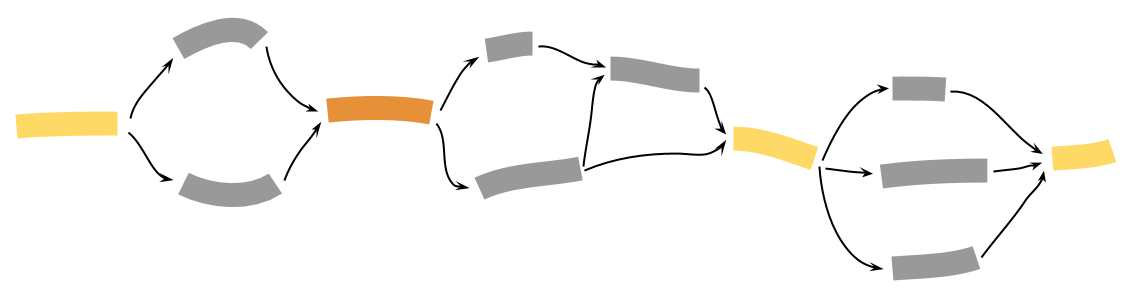
\includegraphics[width=0.8\textwidth]{pics/bubbles_chain.png}
\caption{Цепочка пузырей. Если оранжевая вершина принадлежит штамму, то жёлтые тоже должны ему принадлежать.}
\label{bubbles_chain}
\end{figure}


\begin{figure}[t]
\centering
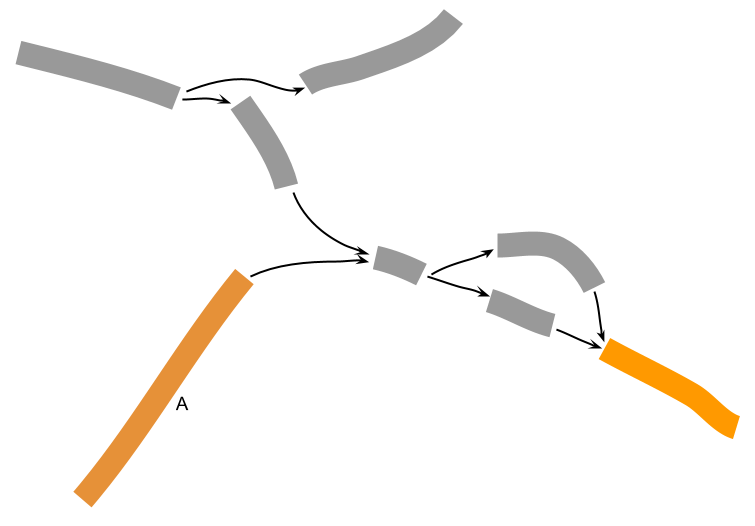
\includegraphics[width=0.57\textwidth]{pics/one_continue.png}
\caption{У вершины $A$ только одно продолжение}
\label{one_continue}
\end{figure}


\subsection{Пузыри в графе}

Было отмечено, что значительная часть развилок соответствует началу вариабельных геномных регионов, представляющих отличия между штаммами.

Большая часть таких отличий соответствует в графе так называемым <<суперпузырям>> -- направленным ациклическим подграфам с выделенными вершинами <<начала>> и <<конца>>). Говоря неформально, пути, выходящие из такой развилки, могут идти по разным вершинам, но потом вновь сходятся в одну (более строгое определение будет дано ниже). Важное наблюдение заключается в том, что начало и конец пузыря должны принадлежать одному и тому же набору штаммов (в частности конец также принадлежит штамму S). 

Следуя работе \cite{superbubbles}, мы определяем понятие \textit{суперпузыря} таким образом --- если упорядоченная пара вершин $(s,t)$ удовлетворяет следующим свойствам:
\begin{enumerate}
    \item $t$ достижима из $s$;
    \item набор вершин, достижимых из $s$ без прохождения через вершину $t$ равняется набору вершин, из которых достижима $t$ без прохождения через вершину $s$;
    \item подграф, индуцированный набором $U$ вершин из предыдущего условия, --- ацикличен;
    \item ни одна вершина из $U$, кроме $t$, не образует с $s$ пары, удовлетворяющей предыдущим условиям;  
\end{enumerate}
то тогда множество вершин $U \cup \{s,t\}$ образуют \textit{суперпузырь}, а $s$ и $t$ --- это его начало и конец соответственно.

Авторы \cite{superbubbles} также предложили простой алгоритм, основанный на топологической сортировке, который для каждой вершины за константное время в среднем определяет, является ли она началом \textit{суперпузыря} $s$, и если это так, то возвращает его конец и множество U.

Таким образом, мы стартуем от вершины V, принадлежащей штамму S, и проверяем, удовлетворяет ли она одному из двух условий:
\begin{enumerate}
    \item Равна ли исходящая степень вершины 1? Если да, помечаем её единственного соседа тоже как принадлежащего штамму S и переходим к нему.
    \item Является ли вершина V началом пузыря? Если да, помечаем конец пузыря тоже как принадлежащий штамму S и переходим к нему, <<перепрыгивая>> таким образом пузырь (см. Рис. \ref{bubbles_chain}). 
\end{enumerate}
Так мы можем повторять эту процедуру итеративно до тех пор, пока путь не остановится в вершине, не подходящей ни под одно из условий. То же самое мы делаем по обратным рёбрам графа.

\subsection{Глубокий анализ пузырей}

После того, как мы добавим к классификации концов пузырей недостающие штаммы, мы можем сказать, какое подмножество штаммов должно проходить через каждый из найденных пузырей. Тогда мы можем уточнить классификацию вершин внутри пузыря, основываясь на их покрытии.

Каждый штамм в пузыре соответствует пути между его началом и концом. Заметим, что мы ищем только пузыри, представляющие из себя направленные ациклические подграфы, поэтому пути в них будут простыми (проходящими по каждой вершине не более одного раза). Мы можем перебрать все варианты путей и их соответствий штаммам, чтобы найти, какой набор путей наилучшим образом объясняет наблюдаемые покрытия вершин. Заметим, что количество возможных путей растёт экспоненциально с увеличением числа вершин в пузыре, поэтому таким образом мы не сможем обрабатывать пузыри, содержащие большое количество вершин.

Пусть через пузырь проходит $k$ штаммов, бинарная матрица $\Theta$ описывает, какому набору штаммов принадлежит каждая из вершин в текущем варианте, $\theta_{v}^{s} = 1$, если штамм $s$ проходит через вершину $v$. 

Пусть $P$ --- вектор длины $k$, отражающий пропорции штаммов, присутствующих в пузыре. Его мы посчитаем, зная ответ DESMAN о пропорциях всех штаммов.

Посчитаем, какую долю от среднего покрытия составляет покрытие каждой из вершин. Чтобы узнать среднее покрытие в пузыре, возмём взвешенное среднее покрытий вершин $s$ и $t$, где $s$ и $t$ --- начоло и конец пузыря, а веса --- их длины, то есть $$cov_{bubble} = \frac{cov_s l_s + cov_t l_t}{l_s + l_t}$$
Тогда наблюдаемая доля от общего покрытия в вершине $v$ будет $$p_{v}^{(0)} = cov_{v} / cov_{bubble}$$
Теоретическая доля от общего покрытия в вершине $v$ будет $$p_{v}^{(1)} = \sum_{s=1}^{k} \theta_{v}^{s} P_s$$
Тогда введём следующую ошибку для рассматриваемого варианта:
$$error = \sum_{v \in bubble} ||p_{v}^{(0)} - p_{v}^{(1)}||_2 \ln l_{v}$$
Множитель $\ln l_v$ нужен нам для того, чтобы учитывать сильнее ошибки, получившиеся на более длинных вершинах, так как их покрытие мы считаем более достоверным.

Таким образом мы считаем, что вариант путей, имеющий наименьшую ошибку, лучше всего описывает наблюдаемые покрытия вершин.

Задача, схожая с поставленной, рассматривалась в серии работ, посвященных реконструкции альтернативных изоформ эукариотических генов на основании серий экспериментов транскриптомного секвенирования (RNA-seq) \cite{flipflop2, other_flows, flipflop1}. Как здесь нам нужно определить, какому набору штаммов принадлежит вершина, так при РНК-секвенировании нужно находить, в какие изоформы входит тот или иной экзон. В данных работах активно используется максимизация правдоподобия пуассоновских процессов. Мы попробовали такой подход на наших данных, но он показал результат хуже.


%\subsection{Итоговый алгоритм}
% * <novmargo@gmail.com> 06:58:17 09 Jun 2018 UTC+0300:
% TODO

%ОФОРМИТЬ ВСЁ ВЫШЕСКАЗАННОЕ В ПСЕВДОКОД



\section{Результаты}
\subsection{Простые датасеты из смесей изолятов}
Графики, по которым предполагается определять количество штаммов, представлены на Рис. \ref{fig:sim_dev}. Видно, что график перестаёт убывать на том количестве штаммов, которое мы ожидаем, везде, кроме образца g2\_r2. 

Во всех экспериментах DESMAN весьма точно определил процентное соотношение штаммов. Усредненная ошибка по всем штаммам во всех образцах для каждого эксперимента приведена в таблице \ref{res_table}.

Также в таблице \ref{res_table} приведены средние точность и полнота классификации вершин графа после каждого этапа пайплайна. Видно, что точность после каждого шага остаётся очень высокой, в то время как полнота растёт, так как мы прибавляем к ответу ранее не классифицированные вершины.


\begin{figure}
    \centering
    \begin{subfigure}[b]{0.3\textwidth}
        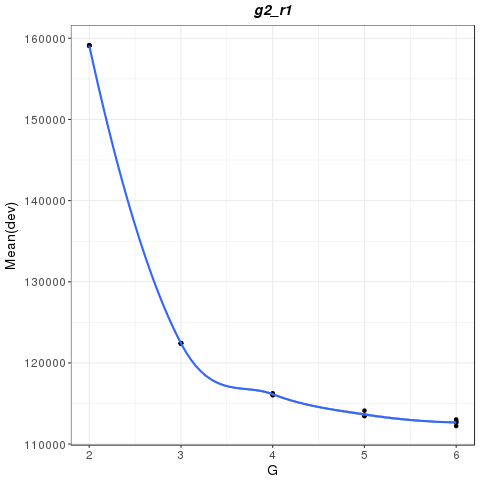
\includegraphics[width=\textwidth]{pics/devs/g2_r1.png}
    \end{subfigure}
    \qquad
    \begin{subfigure}[b]{0.3\textwidth}
        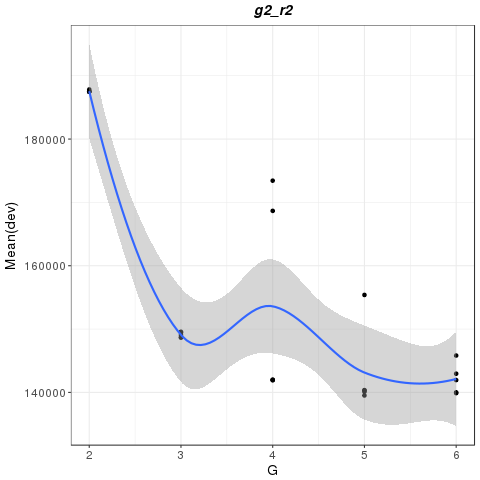
\includegraphics[width=\textwidth]{pics/devs/g2_r2.png}
    \end{subfigure}
      
    \hfill
      
   \begin{subfigure}[b]{0.3\textwidth}
        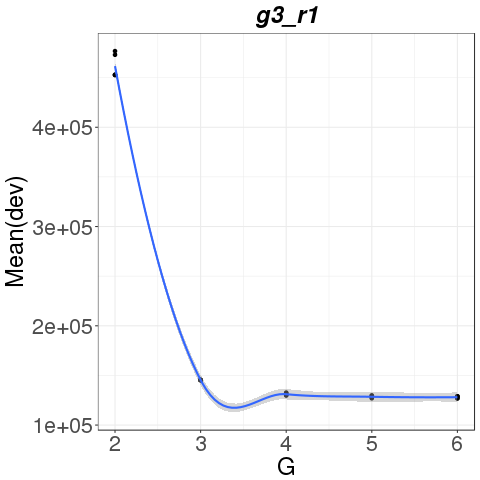
\includegraphics[width=\textwidth]{pics/devs/g3_r1.png}
    \end{subfigure}
    \qquad
    \begin{subfigure}[b]{0.3\textwidth}
        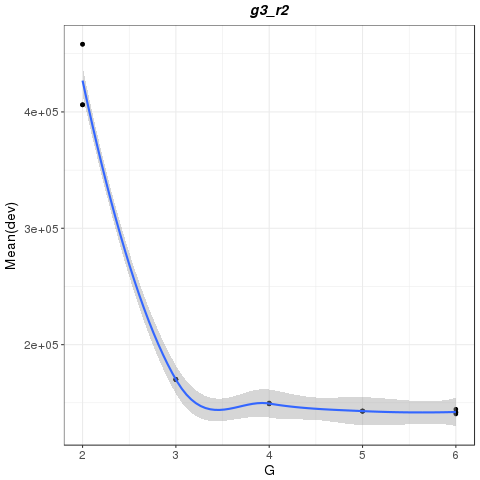
\includegraphics[width=\textwidth]{pics/devs/g3_r2.png}
    \end{subfigure}
      
    \hfill
      
   \begin{subfigure}[b]{0.3\textwidth}
        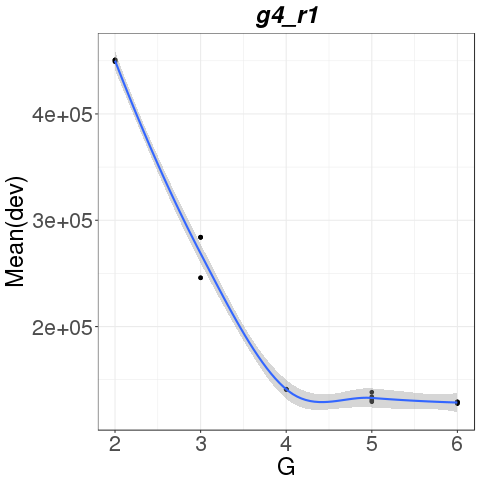
\includegraphics[width=\textwidth]{pics/devs/g4_r1.png}
    \end{subfigure}
    \qquad
    \begin{subfigure}[b]{0.3\textwidth}
        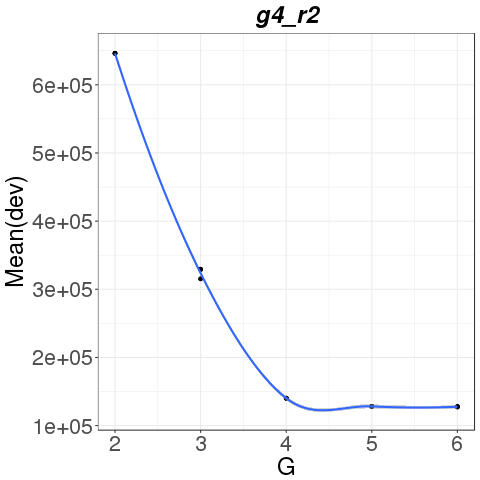
\includegraphics[width=\textwidth]{pics/devs/g4_r2.png}
    \end{subfigure}
      
    \hfill
      
   \begin{subfigure}[b]{0.3\textwidth}
        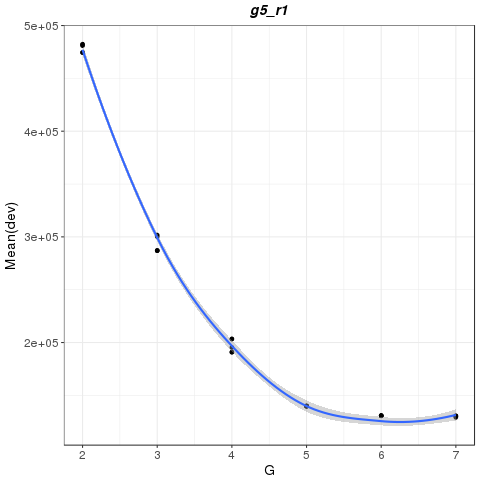
\includegraphics[width=\textwidth]{pics/devs/g5_r1.png}
    \end{subfigure}
    \qquad
    \begin{subfigure}[b]{0.3\textwidth}
        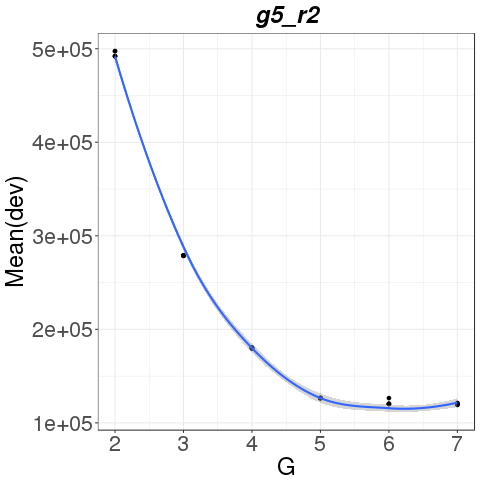
\includegraphics[width=\textwidth]{pics/devs/g5_r2.png}
    \end{subfigure}
    
    \caption{Среднее апостериорное отклонение в зависимости от количества штаммов в синтетических данных.}
    \label{fig:sim_dev}
\end{figure}


\begin{table}[]
\centering
\begin{tabular}{@{}lllllll@{}}
\toprule
эксперимент & \begin{tabular}[c]{@{}l@{}}средняя\\ ошибка\\ частот\\ штаммов\end{tabular} &  &  & \begin{tabular}[c]{@{}l@{}}DESMAN \\ на юнитигах \\ \textgreater 1kb\end{tabular} & \begin{tabular}[c]{@{}l@{}}дополнение \\ однозначных \\ продолжений\end{tabular} & \begin{tabular}[c]{@{}l@{}}анализ \\ пузырей\end{tabular} \\ \hline \midrule
g2\_r1 & 0.002 &  & precision & 0.99 & 0.99 & 0.99 \\
 &  &  & recall & 0.67 & 0.83 & 0.91 \\\hline
g2\_r1 & 0.021 &  &  & 0.98 & 0.98 & 0.99 \\
 &  &  &  & 0.44 & 0.57 & 0.78 \\\hline
g3\_r1 & 0.011 &  &  & 0.99 & 0.99 & 0.99 \\
 &  &  &  & 0.52 & 0.71 & 0.85 \\\hline
g3\_r2 & 0.024 &  &  & 0.98 & 0.97 & 0.97 \\
 &  &  &  & 0.51 & 0.69 & 0.81 \\\hline
g4\_r1 & 0.015 &  &  & 0.99 & 0.98 & 0.99 \\
 &  &  &  & 0.40 & 0.58 & 0.76 \\\hline
g4\_r2 & 0.015 &  &  & 0.99 & 0.98 & 0.98 \\
 &  &  &  & 0.38 & 0.55 & 0.79 \\\hline
g5\_r1 & 0.008 &  &  & 0.97 & 0.96 & 0.97 \\
 &  &  &  & 0.26 & 0.41 & 0.67 \\\hline
g5\_r2 & 0.025 &  &  & 0.99 & 0.99 & 0.99 \\
 &  &  &  & 0.26 & 0.42 & 0.67 \\\hline
\begin{tabular}[c]{@{}l@{}}infant\\ gut\end{tabular} &  & s1 & \begin{tabular}[c]{@{}l@{}}precision\\ recall\end{tabular} & \begin{tabular}[c]{@{}l@{}}0.76\\ 0.22\end{tabular} & \begin{tabular}[c]{@{}l@{}}0.76\\ 0.43\end{tabular} & \begin{tabular}[c]{@{}l@{}}0.77\\ 0.51\end{tabular} \\
 &  & s3 & \begin{tabular}[c]{@{}l@{}}precision \\ recall\end{tabular} & \begin{tabular}[c]{@{}l@{}}0.82\\ 0.21\end{tabular} & \begin{tabular}[c]{@{}l@{}}0.85\\ 0.40\end{tabular} & \begin{tabular}[c]{@{}l@{}}0.86\\ 0.48\end{tabular} \\ \bottomrule
\end{tabular}
\caption{Результаты экспериментов. Для синтетических данных приведены средние полнота и точность по всем штаммам. Для \textit{infant gut} точность и полнота указаны для двух штаммов отдельно.}
\label{res_table}
\end{table}

%\subsection{Датасет Strain Mock}


\subsection{Реальный датасет} \label{infant_gut_section}

В данном исследовании \cite{infant_gut} авторы нашли в рассматриваемых образцах три штамма S.epidermidis. Авторы посчитали процентное соотношение этих штаммов и сделали качественные сборки двух из них (strain1 и strain3).
% * <novmargo@gmail.com> 11:54:15 09 Jun 2018 UTC+0300:
% (НАПИСАТЬ, КАКИМ ОБРАЗОМ)

В предыдущей работе, до того, как была опубликована статья про DESMAN, мы уже анализировали частоты SNVs, чтобы определить процентное соотношение штаммов. Мы кластеризовали профили частот и смотрели на центры кластеров --- можно ли центры одних кластеров представить как сумму других, соответствующих мутациям только одного штамма. Наш анализ выявил, что в данных присутствует четыре штамма, а профили частот в некоторых образцах отличаются от заявленных в исследовании (см. Рис. \ref{infant_gut_figs}). Анализ с помощью DESMAN подтвердил наши результаты. Кроме того мы нашли в графе сборке две длинные вершины , которые не выравниваются на strain1 и strain3, но судя по выравниванию на базу NCBI точно принадлежат S.epidermidis, и их покрытие также соотносится с нашими результатами.
% * <novmargo@gmail.com> 11:55:58 09 Jun 2018 UTC+0300:
% (УКАЗАТЬ ДЛИНУ)
% * <novmargo@gmail.com> 11:55:08 09 Jun 2018 UTC+0300:
% (НАПИСАТЬ ЕЩЕ, ЧТО 36 ГЕНОВ НЕ ОК)

Из графа сборки этих данных не получается однозначно выделить компоненту, принадлежащую S.epidermidis, так как в образцах присутствует родственный ему вид. Поэтому, чтобы уменьшить потенциальное количество вершин, мы сделали следующее: мы провели биннинг длинных вершин (больше 1000 баз) с помощью CONCOCT. Дальше мы выравняли сборки из статьи на граф и выкинули те длинные вершины, которые не выравнивались на S.epidermidis и принадлежали бинам, в которых его было меньше 30\%. После этого мы оставили только компоненту слабой связности, которой принадлежали все вершины S.epidermidis. В получившемся графе мы удалили все короткие тупики (меньше 500 баз) и сжали вместе все вершины, которые можно было соединить. Таким образом мы сузили количество рассматриваемых вершин и упростили граф, но, скорее всего, не потеряли вершины, которые принадлежат S.epidermidis. Выравнивание длинных вершин на базу NCBI показало, что мы включили в анализ как вершины, принадлежищие S.epidermidis (но которых нет в сборках статьи), так и вершины плазмид и фагов S.epidermidis, плюс небольшое количество вершин родственного вида. Но нашей целью является поиск штаммо-специфичных вариаций, которые могли бы в дальнейшем объяснить фенотипические различия, поэтому мы исходим из того, что лучше добавить в анализ лишние вершины, чем потерять нужные.
% * <novmargo@gmail.com> 11:54:38 09 Jun 2018 UTC+0300:
% ???

Чтобы оценить качество наших результатов, мы выравнили на граф strain1 и strain3. В табличке \ref{res_table} представленны результаты для них. Видно, что точность сильно упала, по сравнению с синтетическими датасетами, но это из-за того, что в граф попали вершины не S.epidermidis. 

\begin{figure}
    \centering
    \begin{subfigure}[b]{0.7\textwidth}
        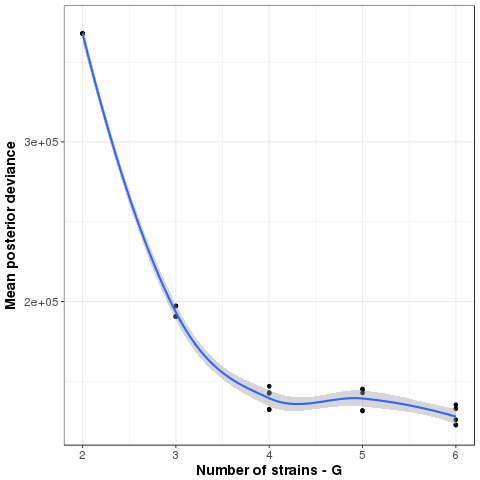
\includegraphics[width=\textwidth]{pics/infant_gut_dev.png}
        \caption{Среднее апостериорное отклонение}
    \end{subfigure}
      
    \hfill
      
    \begin{subfigure}[b]{1.0\textwidth}
        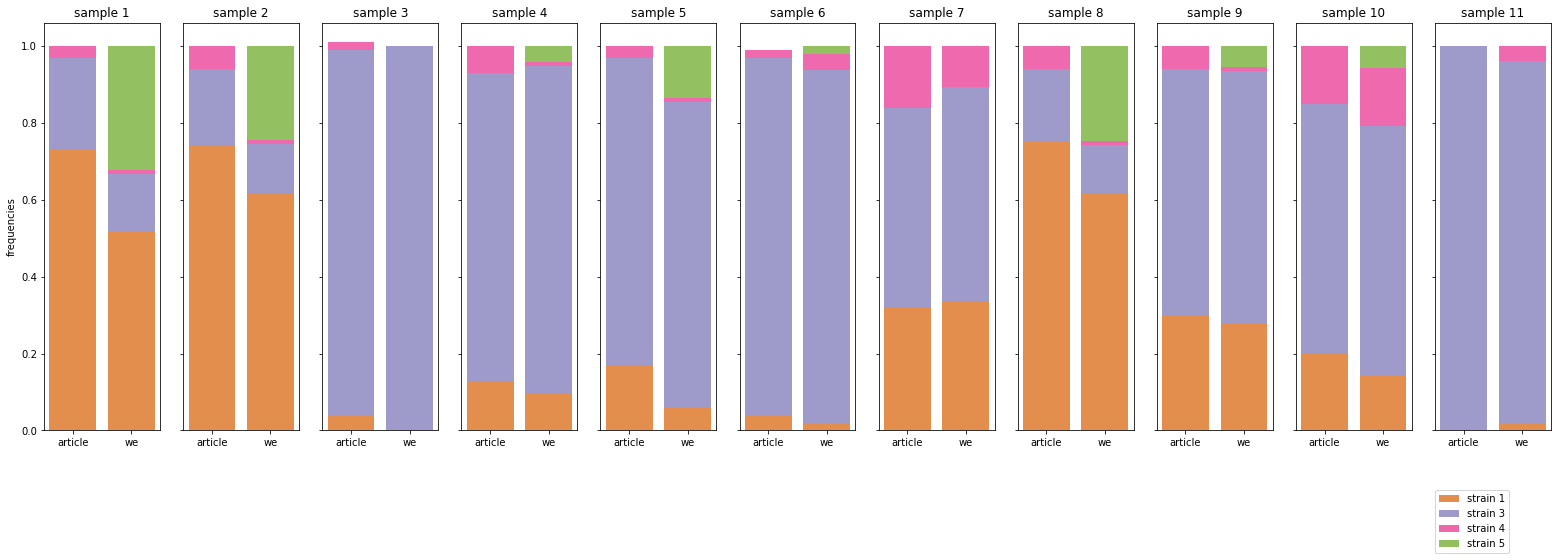
\includegraphics[width=\textwidth]{pics/infant_gut_results.png}
        \caption{Сравнение получившихся частот с оригинальным исследованием}
    \end{subfigure}
    
    \caption{количество и пропорции штаммов \textit{S.epidermidis} в \textit{infant gut}}\label{infant_gut_figs}
\end{figure}


% У заключения нет номера главы
\section*{Заключение}
...






\bibliographystyle{ugost2008ls}
\bibliography{diploma.bib}

%\appendix
\begin{appendices}

\section{Поиск смесей штаммов в образцах}\label{dominated_samples}

ПЕРЕПИСАТЬ

Опишем алгоритм поиска образцов с доминантными штаммами некоторого рассматриваемого вида.

В каждом образце найдем однонуклеотидные мутации относительно референса рассматриваемого вида. Для каждой мутации считаем, сколько ридов поддерживает референс, а сколько – мутацию. Чтобы оставить только те мутации, которые не лежат в повторах и малопокрытых участках генома, возьмем только такие, чье суммарное покрытие близко к медиане покрытия этого вида в образце. Для каждой из выбранных мутаций подсчитаем частоту ридов, поддерживающих мутацию.

Каждая мутация специфична для какого-то одного штамма или некоторого множества штаммов. Если мы выбрали мутации с хорошим покрытием и не попадающие в повторы, то частота ридов, поддерживающих эту мутацию, должна примерно соответствовать сумме частот штаммов, для которых специфична эта мутация.

Тогда заметим, что если частота доминантного штамма – X, и X > 0.7, то мы должны наблюдать мутации с частотой порядка X и больше. При этом мутации, специфичные только для всех остальных штаммов, не могут давать частоты больше (1-X). Тогда в случае, когда в образце присутствует доминантный штамм, в распределении частот, соответствующих мутациям, мы должны наблюдать отсутствие значений в промежутке ((1-X); X).

Найдем величину промежутка эмпирически. Так как границы промежутка должны быть симметричны относительно значения 0.5, начнем с его середины и будем добавлять с обоих концов некоторую маленькую величину eps (например, 0.01) до тех пор, пока в промежуток попадает не больше 5\% от всех значений частот мутаций (те мутации, которые туда попали, считаем погрешностью). После того, как мы нашли предполагаемый промежуток, смотрим на его правую границу. Если она больше 0.7, считаем, что X > 0.7, и в образце есть доминантный штамм. Иначе – доминантного штамма нет.


\section{приложение два}
текст

\end{appendices}

\end{document}
